% referencial_teorico.tex

\pagebreak
\chapter{Referencial teórico}
\index{Referencial Teórico}

\pagebreak
\section{Recuperação de informação}
\index{Recuperação de informação}

Um sistema de recuperação de informações (SRI) é um sistema capaz de armazenar, obter e dar manutenção em informações \cite[p. 2]{kowalski}. Neste contexto, informação pode composto por texto, imagens, audio, vídeo e outros objetos multimídia.

Um SRI consiste em um programa de software que facilita a busca de informação por um usuário. O grau de sucesso de um SRI é dado no quanto o mesmo diminui a burocracia (\emph{overhead}) para o usuário encontrar uma informação. O sucesso de um SRI é muito subjetivo e baseia-se em qual informação que o usuário quer e sua predisposição a enfrentar ou não a burocracia do processo \cite[p. 4]{kowalski}

\subsection{SRIs para Web}
\index{Recuperação de informação!SRIs para Web}

Comparado com SRIs clássicos, os SRIs para Web encara conjunto de dados totalmente diferentes \cite[p. 2]{surveyir}. Segundo \cite{surveyir}, dentre os motivos que tornam únicos os SRIs para Web, pode-se citar:

\begin{itemize}
	\item \textbf{Internet Dinâmica} - A Internet muda a cada dia enquanto a maioria dos SRIs clássicos são feitos para bancos de dados estáticos.
	\item \textbf{Heterogenidade} - A Internet contém uma grande variedade de tipos de documentos: figuras, arquivos de áudio, textos, scripts, etc.
	\item \textbf{Variedade de línguas} - O número de línguas diferentes na Internet passa de 100.
	\item \textbf{Duplicação} - A cópia é uma outra característica importante da Web, em que há estimativas que a quantidade de conteúdo copiado chega a 30\% \cite{surveyir}.
	\item \textbf{Alto número de links} - Em média, cada documento tem mais que 8 links para outras páginas.
	\item \textbf{Consultas heterogêneas} - SRIs para Web têm que lidar com pequenas consultas e não necessariamente bem representadas dos usários de Internet.
	\item \textbf{Grande variância de usuários} - Cada usuário da Web é diferente em vista das suas necessidades, resultados esperados e conhecimento.
	\item \textbf{Comportamento específicos} - É estimado que cerca de 85\% olham somente na primeira página dos resultados retornados dos motores de busca. 78\% dos usuários nunca modificam seu primeiro termo de consulta.
\end{itemize}

Sendo assim, é possível concluir que o grande desafio de SRIs para Web é suprir as necessidades de informação dos usuários dado a heterogenidade da Web.

\subsubsection{Motores de busca de propósito geral}
\index{Recuperação de informação!SRIs para Web!Motores de busca de propósito geral}

Dentre os motores de busca de propósito geral mais utilizados, pode-se citar o Google, Bing e o AltaVista. Dentre os principais objetivos de um motor de busca de propósito geral pode-se destacar: 

\begin{itemize}
	\item Resultados de qualidade, independentemente da consulta utilizada.
	\item Uma boa cobertura dos documentos disponíveis na Web.
	\item Facilidade de uso.
	\item Ser agnóstico quanto ao tipo de mídia e documento a ser pesquisado.
\end{itemize}

Todos os serviços citados anteriormente estão de acordo com as necessidades dispostas acima. Devido à natureza destes motores de busca, é difícil, buscar por somente uma informação em específico, como "Altura em centímetros do Michael Jordan". O máxmimo que estes motores podem fazer é retornar uma página que possa conter esta informação, não a informação em si.

\subsubsection{Motores de busca de domínio específico}
\index{Recuperação de informação!SRIs para Web!Motores de busca de domínio específico}

Ao contrário dos motores de busca de propósito geral, que buscam informações em sites sem distinção, os motores de busca de domínio específico buscam por informações específicas em sites específicos.

Tais motores de busca podem ser utilizados para suprir a necessidade de precisão que se perde com os motores de busca de propósito geral, fornecendo ao usuário resultados mais completos, relevantes e/ou específicos.

Motores de busca de domínio específico estão se tornando populares porque oferecem uma melhor precisão com recursos extra que não são possíveis com motores de busca de propósito específico \cite[p. 8]{wober}.

Um outro problema com grandes motores de busca é sua falha em manter índices atualizados, que é um resultado do vasto número de páginas que precisam ser indexadas. Um motor de busca de propósito específico possui um conjunto menor de páginas para indexar e consequentemente podem atualiza-las mais frequentemente, o que leva a resultados mais atualizados para os usuários.

A funcionalidade extra se refere à apresentação de interfaces mais sofisticadas para usuários que são configurados para um domínio particular de busca. Desde que todos os usuários visitando uma busca de domínio específico pertecem a um grupo de pessoas com interesses e desejos similares, a busca específica por domínio pode utilizar mais efetivamente o perfil do usuário para dar recomendações mais precisas quando o mesmo tiver dificuldades de especificar suas necessidades \cite[p. 9]{wober}.



\subsection{Web crawlers e web scrapers}
\index{Recuperação de Informação!Web crawlers e web scrapers}

\emph{Web crawlers} ou \emph{spiders} são programas de computador que navegam pela World Wide Web de maneira metódica e automatizada \cite{herberth}.

Dentre os \emph{web crawlers} mais famosos, pode-se destacar o GoogleBot, o Yahoo! Slurp e o MSNBot.

\pagebreak
\section{Python}
\index{Python}

\subsection{Histórico}
\index{Python!Historico}
Segundo \cite{pythondoc}, o Python é uma linguagem poderosa, de propósitos gerais, fácil de aprender e programar, interpretada, orientada a objetos e com alguns outros atributos que a tornam uma linguagem ideal para \emph{scripting} e desenvolvimento rápido de aplicações.

A linguagem Python foi criada no início dos anos 1990 por Guido Van Rossum \cite{pythonlicense}, no Stichting Mathematisch Centrum, na Holanda, com o intuito de ser uma linguagem substituta ao ABC, que apresentava uma série de problemas, especialmente com estensibilidade \cite{pythonfaq}. A linguagem Python, inicialmente, foi criada para ser uma substituta da linguagem ABC e com os poderes da API 

Van Rossum permanece como o principal autor da linguagem Python, apesar de receber várias contribuições de colaboradores externos.

Um erro comum é associar a origem o nome da linguagem Python com o nome da serpente. De fato, Van Rossum se inspirou num grupo de comediantes britânicos, o Monty Python, para dar nome à linguagem \cite{pythonfaq} . %referencias?


%colocar mais sobre o histórico

\subsection{Características}
\index{Python!Caracteristicas}
Qualidade de software, produtividade do programador, portabilidade, bibliotecas de suporte, integração de componentes e diversão, são os principais motivos do uso da linguagem \cite{learningpython}. % colocar página 48 e 49

Em seu \emph{design}, o Python implementa uma sintaxe deliberadamente simples e legível e um modelo de programação coerente \cite{learningpython}. %página 50

Dentre as razões históricas, a linguagem Python foi concebida no início da década de 1990, quando ocorreu o \emph{boom} da Internet e quando o número de programadores se tornou escasso para a demanda de Software. Enquanto linguagens de baixo nível como Assembly ou C focam em \emph{produtividade de máquina}, Python foca em \emph{produtividade do programador}. 

Python é deliberadamente otimizada para produtividade do programador. Recursos como sintaxe simples, tipagem dinâmica, falta de necessidade de compilação e um conjunto de ferramentas embutidas permitem que programadores desenvolvam programas em uma fração de tempo necessária em comparação a quando usam outras ferramentas \cite{learningpython}. % página 50

Entretanto, existe um \emph{tradeoff} no uso da linguagem Python: a velocidade de execução. Programadores tendem a ser mais produtivos com o uso de linguagens com os atributos que Python possui. Porém, o código Python não é um código de máquina, portanto o mesmo precisa ser interpretado a cada execução, o que o torna mais lento. 

Outros fatores como a tipagem dinâmica tendem a trazer mais \emph{overhead} na execução dos programas em Python, o que degrada ainda mais sua velocidade de execução, o que torna seu uso difícil ou inviável para projetos que dependam estritamente de velocidade de execução (ex: componentes de baixo nível, como Kernels e drivers de dispositivos, aplicativos de produtividade, como suítes de escritórios e CAD e outros softwares de grande porte).

\subsubsection{Tipagem dinâmica}
\index{Python!Ambientes e plataformas!Tipagem Dinâmica}

A tipagem dinâmica é uma propriedade de uma linguagem de programação que permite que a checagem de tipo seja feito em tempo de execução, em detrimento da tipagem estática, onde a verificação de tipo é feita em tempo de compilação.

Segundo \cite{dynamic_langs}, as principais vantagens ao se utilizar uma linguagem de tipagem dinâmica é evitar a rigidez de linguagens estaticamente tipadas, tornar mais fácil a prototipação de sistemas que possuem requisitos ainda não conhecidos ou que mudam de uma forma não previsível, aumentar o reuso de código, diminuir a verbosidade e o custo do projeto, sem necessariamente ser menos seguras que as linguagens de tipagem estática.

Devido à seu baixo nível de burocracia e alto poder de prototipação, as linguagens dinâmicas são freqüentemente usadas como "cola" entre componentes \cite{scripting}. Por este motivo, as linguagens dinâmicas também são conhecidas por \emph{glue languages} ou \emph{system integration languages}.

Uma linguagem que não é apegada a tipos permite que a integração entre componentes seja bem mais fácil, pois não há restrições primárias sobre como os retornos de cada componente devam ser utilizados: todos eles são apresentados de uma única forma \cite{scripting}.

Linguagens dinâmicas, como o Python, são ideais para pesquisas e provas de conceito, graças a seu alto poder de prototipação, o que ajuda a explicar o quão Python está em uso na comunidade científica, como demonstrado em \cite{python_scientific_world}.

\subsection{Ambientes e plataformas}
\index{Python!Ambientes e plataformas}

Python é uma linguagem portável e multiplataforma. Isso significa que um código em Python pode ser executado nos mais diversos ambientes e sistemas operacionais, como Windows, Linux, Mac OS e em até sistemas operacionais móveis como Symbian e Android.

Há também a possibilidade de executar a linguagem Python em outros ambientes diferentes do original (CPython). Iniciativas como Jython (Python para a \emph{Java Virtual Machine}) e o IronPython (Python para o ambiente Microsoft.NET) permitem que o Python seja executado dentro das duas das maiores plataformas de desenvolvimento de software da atualidade, aproveitando seus recursos e suas funcionalidades. 

Desta forma, um programa em Python pode utilizar o Swing através do Jython para o desenvolvimento de uma interface gráfica em ambiente Java ou pode utilizar o \emph{Windows Communication Foundation} como \emph{framework} de troca de mensagens no ambiente Microsoft.NET.

\subsubsection{CPython}
\index{Python!Ambientes e plataformas!IronPython}

O CPython é a implementação padrão da linguagem Python e é escrita na linguagem de programação C \cite[p.6]{pypy}. A linguagem é implementada por um compilador que traduz código Python em um código \emph{bytecode} de altíssimo nível (\emph{very high level}) e por uma máquina virtual que interpreta o código.

\subsubsection{IronPython}
\index{Python!Ambientes e plataformas!IronPython}

O IronPython \cite{ironpython} é uma implementação da linguagem de programação Python que é execuatada no framework .NET e Silverlight. Suporta um shell interativo (como a maioria das implementações da linguagem Python) com completa compilação dinâmica. É bem integrado com o resto do framework .NET e torna todas as bibliotecas do .NET facilmente disponíveis para programadores Python, enquanto mantém a compatibilidade com a linguagem Python.


\subsubsection{Jython}
\index{Python!Ambientes e plataformas!Jython}

Jython \cite{jython} é uma implementação da linguagem Python para a JVM (\emph{Java Virtual Machine}). O Jython torna possível a execução da sintaxe da linguagem de programação Python na plataforma Java, o que permite uma integração transparente com as bibliotecas Java e outras aplicações baseadas em Java. 

\subsubsection{PyPy}
\index{Python!Ambientes e plataformas!PyPy}

PyPy é uma implementação do Python escrita em Python \cite[p. 7]{pypy}. A idéia principal é escrever uma especificação de alto nível do interpretador em um subtrato restrito do Python chamado RPython (\emph{Restricted Python}) com o intuito de ser traduzido para executáveis eficientes de baixo nível para o ambiente C/POSIX, JVM e CLI, o que garante a portabilidade. 

\subsection{Python e Computação Científica}
\index{Python!Python e Computação Científica}

Segundo \cite{python_scientific_world}, Python e estensões como o NumPy \cite{numpy} estão se tornando padrão para muitas ciências que precisam processar grande quantidades de dados, desde a neuroimagem à astronomia.

Conferências anuais especificamente voltadas para usos de Python em computação científica, como o SciPy \cite{scipy} (tanto na versão norte-americana quanto na européia) vem ganhando peso a cada ano.

Ambientes de desenvolvimento integrado como o PythonXY \cite{pythonxy} ajuda a mostrar para cientistas que a linguagem Python com seus pacotes de bibliotecas e softwares para computação científica pode ser uma excelente alternativa para ambientes como o Matlab.

Um dos casos mais famosos da linguagem Python sistemas de recuperação de informações é o Google.\cite{google}. Python representa um papel fundamental dentro da estrutura de motores de busca do Google, sendo responsável pelos seus \emph{crawlers} e pelos seus servidores de URL \cite{surveyir}.


\pagebreak
\section{Scrapy}
\index{Scrapy}


Scrapy é um framework rápido ede alto nível para \emph{scrren scraping} e \emph{web crawling}, usado para navegar por websites e extrair dados estruturados de suas páginas. Pode ser usado para um grande número de propósitos, desde mineração de dados a monitoramento e automação de testes \cite{scrapy}.

Mesmo que o Scrapy tenha sido originalmente feito para \emph{screen scraping} (mais precisamente para \emph{web scraping}), ele também pode ser usado para extrair dados usando APIs (como as APIs de serviços da Amazon) ou pode ser usado como um \emph{web crawler} de propósito geral.

Dentre as principais funcionalidades que o Scrapy apresenta, pode-se citar:

\begin{itemize}
	\item Suporte embutido para selecionar e extrair dados de fontes em HTML ou XML.
	\item Suporte embutido para limpeza e sanitização dos dados obtidos utilizando uma coleção de filtros reusáveis (chamados de \emph{Item Loaders}) compartilhados entre todos os \emph{web crawlers}.
	\item Suporte embutido para geração e exportação de \emph{feeds} em múltiplos formatos (como JSON, XML e CSV) e armazenamento dos mesmos (seja em FTP ou localmente).
	\item Um \emph{pipeline} de mídia para download automático de imagens (ou qualquer outro tipo de mídia) associado com os itens obtidos.
	\item Suporte para estensão do Scrapy, onde é possível adicionar funcionalidades ao framework através do uso de sinais e uma API bem definida.
	\item Grande quantidade de \emph{middlewares} e estensões para gerenciamento de cookies e sessões, compressão HTTP, autenticação HTTP, cache HTTP, mudança do header \emph{user-agent} e restições sobre a profundidade de \emph{crawling}.
	\item Suporte robusto para auto-detecção de encoding assim como manipulação de encodes estrangeiros, quebrados e fora dos padrões.
	\item Extensa coleção de status para métricas do \emph{crawler}, úteis para monitoramento de performance e de disponibilidade.
	\item Um console interativo para teste de XPaths, úteis para debugging.
	\item Um serviço a nível de sistema feitos para facilitar a implantação e execução dos crawlers em produção.
	\item Webservices e console telnet embutidos para monitoração, controle, introspecção e debugging do crawler.
\end{itemize}

\subsection{Arquitetura}
\index{Scrapy!Arquitetura}

O diagrama a seguir dá uma visão geral da arquitetura do Scrapy com seus componentes e o fluxo de dados que há dentro do sistema (mostrado em setas verdes). Uma breve descrição dos componentes e o fluxo de dados estão incluídos abaixo.

\begin{figure} [ht]
	\centering
	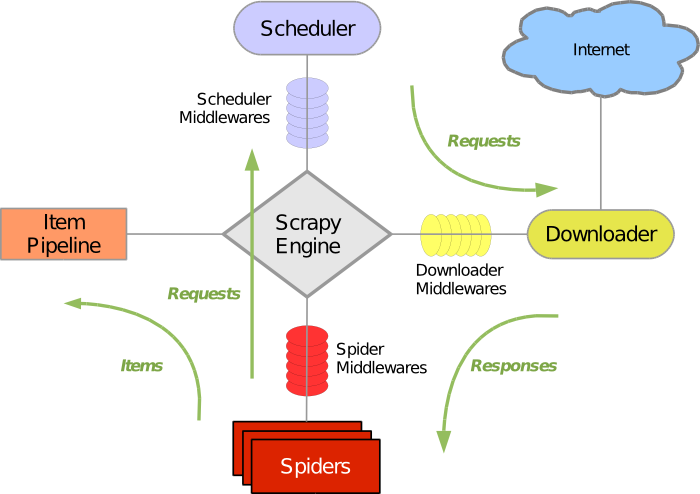
\includegraphics[scale=1]{scrapy_architecture.png}
	\caption{Visão geral da arquitetura do scrapy \cite{scrapy_arch}}
	\label{scrapy_architecture}
\end{figure}

\subsubsection{Scrapy engine}
\index{Scrapy!Arquitetura!Scrapy engine}

O engine é responsável por controlar o fluxo de dados entre todos os componentes do sistema, e disparar eventos quando certas ações ocorrerem.
% colocar mais informações sobre data flow

\subsubsection{Scheduler}
\index{Scrapy!Arquitetura!Scheduler}

O scheduler recebe requisições do engine e as enfileira para realimentação da engine no futuro.

\subsubsection{Downloader}
\index{Scrapy!Arquitetura!Downloader}

O Downloader é responsável por obter páginas da Web e alimetar o engine, que por sua vez alimenta os crawlers/spiders.

\subsubsection{Item pipeline}
\index{Scrapy!Arquitetura!Item pipeline}

O Item Pipeline é responsável para processar os itens uma vez que eles foram extraídos pelos crawlers/spiders. Tarefas típicas do Item Pipeline incluem limpeza, validação e persistência do item.

%colocar mais informações sobre o este item

\subsubsection{Spider middlewares}
\index{Scrapy!Arquitetura!Spider middlewares}

Spider middlewares são \emph{ganchos} específicos que ficam entre a Engine e os Spiders e podem processar a entrada de um sipder (respostas) e saídas (itens e requisições). Eles fornecem um mecanismo conveniente para estender as funcionalidades do Scrapy através da adição de código customizado.

%colocar mais informações sobre o spider middleware

\subsubsection{Scheduler middlewares}
\index{Scrapy!Arquitetura!Scheduler middlewares}

Scheduler middlewares são \emph{ganchos} específicos que ficam entre a Engine e o Schedule e processa requisições quando as mesmas passam do engine para o Scheduler e vice-versa. Eles fornecem um mecanismo conveniente para estender as funcionalidades do Scrapy através da adição de código customizado.

\subsubsection{Fluxo de dados}
\index{Scrapy!Arquitetura!Fluxo de dados}

O fluxo de dados do Scrapy é controlado pela Engine e funciona da seguinte forma:

\begin{enumerate}
	\item Engine abre um domínio, localiza o Spider que manipula aquele domínio e pede para o Spider a primeira URL para navegar.
	\item O Engine pega a primeira URL para navegar do Spider e a agenda no Scheduler como Requisições.
	\item O Engine pede para o Scheduler as próximas URLs para navegar.
	\item O Scheduler retorna a próxima URL para navegação para o Engine e o Engine a manda para o Downloader passando pelo Downloader Middleware.
	\item Uma vez que o download da página terminou, o Downloader gera uma Response (com a página) e a manda para o Engine, passando pelo Downloader Middleware.
	\item O Engine recebe a resposta do downloader e a envia para o Spider processar, passando pelo Spider Middleware.
	\item O Spider processa a Response e retorna os itens obtidos e novas Requests para o Engine.
	\item O Engine envia os itens obtidos (retornados pelo spider) para o Item Pipeline e envia as Requests (retornadas pelo Spider) para o Scheduler.
	\item O processo se repete a partir do passo 2 até que não haja mais Requests no Scheduler e o Engine fecha o domínio.
\end{enumerate}

\subsubsection{E/S orientado a eventos}
\index{Scrapy!Arquitetura!Networking orientado a eventos}

O Scrapy é escrito utilizando o Twisted \cite{twisted}, um framework popular para programação orientada a eventos para Python. Desta forma, ele é implementado utilizado código não-bloqueante (ou assíncrono) para aumentar a concorrência.

\subsection{Serviços embutidos}
\index{Scrapy!Serviços embutidos}

O Scrapy possui uma gama de serviços embutidos feitos para facilitar a monitoração e manutenção do sistema. A seguir, é apresentado cada um destes serviços embutidos bem como uma descrição breve.

\subsubsection{Logging}
\index{Scrapy!Serviços embutidos!Logging}

O log é um histórico de execução do sistema. Através da análise de logs, é possível detectar e achar a fonte de problemas. O Scrapy possui um componente de logging que grava as mensagens de log em um arquivo em disco e possui cinco níveis de log \cite{scrapy_log}:

\begin{enumerate}
	\item \texttt{\textbf{CRITICAL}} - Para erros críticos
	\item \texttt{\textbf{ERROR}} - Para erros regulares
	\item \texttt{\textbf{WARNING}} - Para avisos
	\item \texttt{\textbf{INFO}} - Para mensagens informativas
	\item \texttt{\textbf{DEBUG}} - Para mensagens de debug
\end{enumerate}

O nível de log é configurável e um determinado nível irá catalogar todas as mensagens do nível mais as mensagens dos níveis abaixo. Por exemplo, se o nível de log for configurado para 5 (\texttt{DEBUG}), o sistema irá gravar todas as mensagens de log, ao passo que se o nível de log for configurado para 2 (\texttt{ERROR}), somente as mensagens de erros regulares e erros críticos serão gravados.



\pagebreak
\section{Website Parse Template}
\index{Website Parse Template}


Website Parse Template (WPT) é um formato aberto baseado em XML que fornece informações adicionais a web crawlers como estrutura e conteúdo do HTML. O WPT é compatível com esquemas XML, como o RDF e o OWL \cite{wpt}. É composto por três seções principais:

\begin{itemize}
	\item \textbf{Templates} - Seção mandatória, que contém descrições sobre estrutura e conteúdo de páginas da web em HTML.
	\item \textbf{Ontologia} - Seção opcional que define conceitos e relações usadas em um website.
	\item \textbf{URLs} - Seção opcional, que associa certos padrões de URL para grupos de páginas web para templates específicos. 
\end{itemize}

Cada uma das seções do WPT mostradas acima será discutida a seguir.

\subsection{Seções do WPT}
\index{Website Parse Template!Seções do WPT}

\subsubsection{Templates}
\index{Website Parse Template!Seções do WPT}

A seção de templates descreve a estrutura do HTML fazendo referências aos elementos HTML correspondentes da página em específico \cite{wpt}.

O Template inicia com a tag \texttt{<ow:template>} e termina com  \texttt{</ow:template>}. É obrigatório especificar um nome de template único dentro da tag \texttt{<ow:template>} e definir a URL correspondente ao template específico.

O Template é composto de blocos correspondentes a cada elemento estrutural de uma página web em específico. Cada template precisa ter ao menos um bloco. Um bloco faz referência ao elemento HTML apropriado através de uma ou muitas combinações dos seguintes métodos de referência: TagID, XPath e Pattern. Cada bloco precisa iniciar com uma tag \texttt{<ow:block>} e fechar com \texttt{</ow:block>}. É necessário indicar elementos HTML específicos dentro da tag de abertura do bloco.

\pagebreak
\lstset{language=XML,
basicstyle=\scriptsize,
caption={Exemplo de um Template com três blocos \cite{wpt}},
captionpos=b
}
\begin{lstlisting}
<ow:template ow:name="Template Example" ow:url="http://www.example.com/index.php">
  <ow:block ow:tagid="ex1" ow:xpath="/html/body/div/div" ow:pattern="content (object[[a-z]*])">
    <!--descricao do conteudo -->
  </ow:block>
  <ow:block ow:tagid="ex2">
    <!-- descricao do conteudo -->
  </ow:block>
  <ow:block ow:xpath="/html/body/div/div/table/tr[1]/td">
    <!-- descricao do conteudo -->
  </ow:block>
</ow:template>
\end{lstlisting}

Cada bloco contém o a descrição do conteúdo dos elementos HTML representados isoladamente ou dentro de outro bloco. Blocos embutidos são usados para descrever elementos HTML específicos ("bloco pai") que inclui um ou mais elementos ("bloco filho").

\lstset{language=XML,
basicstyle=\scriptsize,
caption={Exemplo de um Template com blocos embutidos \cite{wpt}},
captionpos=b
}
\begin{lstlisting}
<ow:template ow:name="Template Example" ow:url="http://www.example.com/index.php">

  <ow:block ow:xpath="/html/body/div/div">
    <ow:block ow:xpath="/html/body/div/div/table/tbody/tr[1]/td">
      <!-- descricao do conteudo -->
    </ow:block>
  </ow:block>
  
</ow:template>
\end{lstlisting}

A descrição do conteúdo pode ser informada usando conceitos definidos na seção \emph{Ontology} ou qualquer linguagem/formato suportado: RDF, CWL, etc. É necessário declarar namespaces dos schemas XML usados dentro da tag \texttt{<ow:wpt>} e o nome da ontologia dentro da tag \texttt{<ow:template>}

\pagebreak
\lstset{language=XML,
basicstyle=\scriptsize,
caption={Exemplo de um Template com instâncias de descrição de conteúdo\cite{wpt}},
captionpos=b
}
\begin{lstlisting}
<ow:wpt xmlns:ow="http://www.omfica.org/schemas/ow/0.9"
 xmlns:rdf="http://www.w3.org/1999/02/22-rdf-syntax-ns#"
 ow:host="http://www.example.com">

  <ow:template ow:name="Template Example" ow:url="http://www.example.com/index.php"
   ow:ontology="ontology_example">

     <!-- descricao de conteudo utilizando conceitos definidos -->
     <ow:block ow:tagid="ex1" ow:xpath="/html/body/div/div" ow:pattern="Wellcome (user.name[[A-Za-z]*])">
       conceito_de_ontologia
     </ow:block>
     <!-- descricao de conteudo utilizando a sintaxe RDF -->
     <ow:block ow:tagid="ex2">
       <rdf:Description rdf:about="http://www.example.com/index.php">
       </rdf:Description>
     </ow:block>
     <!-- descricao de conteudo utiliznado CWL.unl -->
     <ow:block ow:xpath="/html/body/div/div/table/tr[1]/td">
       {cwl.unl}
       {/cwl.unl}
     </ow:block>
  </ow:template>

</ow:wpt>
\end{lstlisting}

\subsubsection{URLs}
\index{Website Parse Template!URLs}

Esta seção define as URLS/padrões de URLs das páginas web descritas na seção de Templates. Esta seção é mandatória se os templates não definem as URLs/padrões de URL das páginas web \cite{wpt}.

De acordo com a seção de Templates, esta seção também pode consistir de vários blocos/unidades. Cada um destes blocos iniciam com a tag \texttt{<ow:urls>} e terminam com a tag \texttt{</ow:urls>}.


\lstset{language=XML,
basicstyle=\scriptsize,
caption={Exemplo de padrões de URLs \cite{wpt}},
captionpos=b,
label="wpt_url_pattern"
}
\begin{lstlisting}
\label{lst:wpt_url_pattern}
<ow:urls ow:name="Artist page on Yahoo! Music" ow:template="Artist page on Yahoo! Music">
  <ow:url>http://music.yahoo.com/ar-8206256---Amy-Winehouse</ow:url>
  <ow:url>http://music.yahoo.com/ar-([artist.id[0-9]*])---(artist.name[[A-Za-z0-9-]*])</ow:url>
</urls>
\end{lstlisting}

Especificações utilizando expressões regulares (RegExp) são utilizadas para descrição de padrões de URL. O padrão de URL informado na listagem 1.4 também inclui a real URL representada. Os conceitos necessários para definição de padrões de URL (tais como "id" e "nome") são definidos na seção Ontology.

\subsubsection{Ontology}
\index{Website Parse Template!URLs}

A seção Ontology contém enumerações e definições de todos os conceitos utilizados no website \cite{wpt}. Os conceitos listados precisam ser definidos dentro de das tags \texttt{<ow:ontology>} e \texttt{<ow:ontology>}. É necessário especificar o nome da ontologia dentro da tag \texttt{<ow:ontology>}. O WPT permite tanto o uso de OWL ou da \emph{WPT Ontology language} para definição de conceitos. A principal diferença dentre estas línguas é que a \emph{WPT Ontology language} fornece uma sintaxe simplificada para conceitos e definição de relações.

\lstset{language=XML,
basicstyle=\scriptsize,
caption={Definição conceitual de ''artista'' utilizando a \emph{WPT Ontology language} \cite{wpt}},
captionpos=b,
}
\begin{lstlisting}
<ow:ontology ow:name="general">
  <ow:concept ow:name="artist">
    <ow:inherit>person</ow:inherit>
    <ow:has>name</ow:has>
    <ow:has>album</ow:has>
    <ow:has>track</ow:has>
    <ow:has>image</ow:has>
    <ow:has>bio</ow:has>
    <ow:has>video</ow:has>
    <ow:has>id</ow:has>
  </ow:concept>
  <ow:concept>logo</ow:concept>
  <ow:concept>menu</ow:concept>
  <ow:concept>advertisement</ow:concept>
</ow:ontology>
\end{lstlisting}

Cada definição de conceito inicia com a tag \texttt{<ow:concept>} e termina com a tag\texttt{</ow:concept>}. A tag \texttt{<ow:inherit>} mostra relações de herança e a tag \texttt{<ow:has>} mostra relações atribuíveis entre dois conceitos. Os conceitos definidos tem um atributo padrão - identificador de objeto (id) para ser utilizado por web crawlers para coordenar os mesmos atributos do objeto utilizados em páginas diferentes do mesmo website.

\pagebreak
\section{Protocol Buffers}
\index{Protocol Buffers}

\emph{Protocol Buffers} (ou simplesmente \emph{protobuf})é uma forma de de codificar dados estruturados em um formato eficiente e extensível \cite{protobuf}. 

O \emph{protobuf} foi inicialmente desenvolvido no Google para lidar com um protocolo de requisição/resposta num servidor de índices \cite{protobuf_overview}. Antes do \emph{protobuf}, havia um formato para as requisições e respostas que utilizava uma seleção/desseleção manual e dava suporte à várias versões do protocolo, o que resultava num código difícil de ler, manter e escrever \cite{protobuf_overview} . 

Devido ao versionamento manual do protocolo, havia grandes dificuldades no desenvolvimento e implantação de um novo. Os desenvolvedores precisavam certificar se todos os servidores entre o que origina a requisição e o que manipula a requisição estavam aptos a entender o novo protocolo antes de utiliza-lo \cite{protobuf_overview}.

Segundo \cite{protobuf_overview}, o \emph{protobuf} foi desenvolvido para resolver muitos destes problemas:

\begin{itemize}
	\item Novos campos podem ser facilmente introduzidos e servidores intermediários que não precisavam inspecionar os dados simplesmente o passavam adiante, sem precisar saber sobre todos os campos.
	\item Os formatos eram mais auto-descritíveis e poderiam lidar com uma variedade de linguagens (C++, Java, Python, etc.)
	\item Possuem uma performance superior ao XML, além de serem mais simples e menos ambíguos.
\end{itemize}

\subsection{Esquema de funcionamento}

A informação a ser serializada é espeficada através da definição de mensagens \emph{protobuf} em arquivos \texttt{.proto}. Cada mensagem \emph{protobuf} é um pequeno registro lógico de informação, contendo uma série de pares nome-valor \cite{protobuf_overview} . Eis um exemplo básico de um arquivo \texttt{.proto} que define uma mensagem contendo informações sobre uma pessoa:

\pagebreak
\lstset{language=java,
basicstyle=\scriptsize,
caption={Exemplo de uma mensagem em \emph{protobuf}, que contém informações sobre uma pessoa\label{protobuf_msg}},
captionpos=b,
}
\begin{lstlisting}
message Person {
  required string name = 1;
  required int32 id = 2;
  optional string email = 3;

  enum PhoneType {
    MOBILE = 0;
    HOME = 1;
    WORK = 2;
  }

  message PhoneNumber {
    required string number = 1;
    optional PhoneType type = 2 [default = HOME];
  }

  repeated PhoneNumber phone = 4;
}
\end{lstlisting}


Uma vez que as mensagens foram definidas, é necessario executar o compilador do \emph{protobuf} para a linguagem da sua aplicação no seu arquivo \texttt{protobuf} para que as classes de acesso à dados sejam geradas. Segundo \cite{protobuf_overview}, estas classes fornecem meios de acessos simples para cada campo (como \texttt{query()} e  \texttt{set\_query()}) e métodos para serializar e \emph{parsear} toda a estrutura de e para bytes brutos. Por exemplo, se a linguagem a ser trabalhada fosse C++, executar o compilador \emph{protobuf} no exemplo acima irá fazer com que seja gerada uma classe \texttt{Person}. Esta classe poderia ser usada na sua aplicação para popular, serializar e obter mensagens do tipo \texttt{Person} no estilo \emph{protobuf} e poderia ser utilizada como no exemplo a seguir:

\pagebreak
\lstset{language=C++,
basicstyle=\scriptsize,
caption={Exemplo de uso da classe para C++ gerada a partir da mensagem \texttt{Person}},
captionpos=b,
}
\begin{lstlisting}
// serializacao
Person person;
person.set_name("John Doe");
person.set_id(1234);
person.set_email("jdoe@example.com");
fstream output("myfile", ios::out | ios::binary);
person.SerializeToOstream(&output);	

// deserializacao

fstream input("myfile", ios::in | ios::binary);
Person person;
person.ParseFromIstream(&input);
cout << "Name: " << person.name() << endl;
cout << "E-mail: " << person.email() << endl;
\end{lstlisting}



\subsection{Vantagens sobre outros formatos}

\subsubsection{XML}

São várias as vantagens que o \emph{protobuf} tem sobre o XML. \cite{protobuf_overview} cita algumas:

\begin{itemize}
	\item \emph{protobuf} é mais simples
	\item É de três a dez vezes menor
	\item É De vinte a cem vezes mais rápido
	\item É menos ambíguo
	\item Geram classes de acesso à dados que são mais simples de usar programaticamente
\end{itemize}

Um exemplo é necessário para tornar a ilustração das diferenças do protocol buffer mais óbvias. Suponha que os dados cadastrais de uma pessoa sejam representados em XML desta forma:

\lstset{language=XML,
basicstyle=\scriptsize,
caption={Exemplo de modelagem de dados de uma pessoa utilizando XML},
captionpos=b,
}
\begin{lstlisting}
 <person>
    <name>John Doe</name>
    <email>jdoe@example.com</email>
  </person>
\end{lstlisting}

O código equivalente em \emph{protobuf} seria este:

\lstset{language=XML,
basicstyle=\scriptsize,
caption={Exemplo de modelagem de dados de uma pessoa utilizando \emph{protobuf}},
captionpos=b,
}
\begin{lstlisting}
person {
  name: "John Doe"
  email: "jdoe@example.com"
}
\end{lstlisting}


\subsubsection{JSON}

O JSON (JavaScript Objetct Notation) é um dos principais formatos de troca de dados na Internet hoje. Ele se baseia na forma como são construídos objetos em JavaScript para serialização dos dados. Apesar do nome remeter à uma única linguagem, o JSON pode ser utilizado em várias linguagens e plataformas atuais, como pode ser visto em \cite{json}.

Não foram encontrados comparações diretas com outros formatos de dados além do XML com o \emph{protbuf} em sua documentação oficial, tampouco comparações que fossem agnósticas a plataformas. No entanto, há algumas vantagens naturais que o protobuf oferece:

\begin{itemize}
	\item É mais descritivo, uma vez que suporta vários tipos de mensagens e tipos de dados, enquanto o JSON suporta apenas objetos (ou lista de objetos) em formato chave-valor.
	\item Permite a adição de regras de negócio: um campo dentro de uma mensagem protobuf pode ser opcional, obrigatório ou repetido e pode respeitar à um determinado tipo, seja ele enumeração, inteiro ou string, por exemplo. No JSON, só há a representação dos dados, nada obrigatoriamente descrevendo sua estrutura.
	\item Protocol Buffers podem ser organizados em pacotes \cite{protobuf_docs}, da mesma forma que várias linguagens de programação orientadas a objeto permitem a organização de classes em pacotes ou \emph{namespaces}.
	\item É mais reutilizável e possuem menos \emph{overhead} no armazenamento de dados \cite{twitter_hadoop}.
\end{itemize}

Entretanto, o JSON possui alguns contrapontos em relação ao \emph{protobuf}, o que o faz mais interessantes para sistemas mais heterogêneos (em que vários sistemas escritos em várias linguagens/plataformas precisam se comunicar):

\begin{itemize}
	\item Em comparação com o \emph{protobuf}, é mais fácil extrair informações (\emph{parsear}) do JSON, devido à sua natureza mais simplificada.
	\item É suportado pela maioria das linguagens/plataformas \emph{json}.
	\item Está se tornando rapidamente um padrão na Web, em que iniciativas como o JSON RPC \cite{json_rpc} e a pretenção do Twitter abandonar o XML em detrimento do JSON \cite{twitter_deprecates_xml} provam isso.
\end{itemize}
